\documentclass{article}

\usepackage[english]{babel}
\usepackage[letterpaper,top=3cm,bottom=3cm,left=3cm,right=3cm,marginparwidth=0cm]{geometry}
\usepackage[superscript]{cite} % superscript numeric in-line citations
\usepackage{amsfonts}
\usepackage{lettrine}

% Useful packages
\usepackage{amsmath}
\usepackage{graphicx}
\usepackage[colorlinks=true, allcolors=blue]{hyperref}

\font\myfont=cmr12 at 18pt
\title{{\myfont A Study on the Relationship between the Percentage of Institutional Delivery and the Infant Mortality Rate in India}}
\author{Zhongmang Cheng}
\date{December 20th, 2022}

\begin{document}
\maketitle

\section{Introduction}
With modern technology advances, the infant mortality rate has decreased significantly in developed countries. In Canada, this index has reduced from 40 death per 1000 live births in 1950 to 4.055 death per 1000 live births in 2022\cite{2022UN}. However, in some developing countries, antenatal care and institutional delivery are not widely available. In this research, we will investigate nine states in India. These nine states account for 48\% of the total population and 70\% of infant deaths. We will analyze the statistics of 284 districts and answer the following question: Is the percentage of institutional delivery in a district linearly related to the infant mortality rate in this district?\\

\noindent Existing research mainly focused on using female literacy rates or environmental factors as predictors\cite{gokhale_rao_garole_2022, greenstone_hanna_2011}. A few research studies infant mortality rates on a district level\cite{kapoor_2009}, but only a little research focuses on the potential impact of institutional delivery. The answer to our research question holds importance to developing and undeveloped countries. It could provide a potential guideline for reducing the infant mortality rate.

\section{Methods}
\subsection{Study population}
This analysis was conducted using India's Annual Health Survey (AHS) data from 2012 to 2013. The survey was conducted in Empowered Action Group (EAG) states Uttarakhand, Rajasthan, Uttar Pradesh, Bihar, Jharkhand, Odisha, Chhattisgarh \& Madhya Pradesh, and Assam. More than 20,000 sample unit was collected across 284 districts in these nine states. The original data set contains eight variables and 284 observations. Each observation represents the Mortality and Delivery Care data for each district. 

\subsection{Variable selection}
Two of the eight variables represent the states and the district, which are removed from the analysis as it provides no information on the question we are interested in. Our variable of interest is Infant Mortality Rate. The rest five variables are, therefore, predictors. Among the five predictors, ``Institutional Delivery'' and ``Delivery At Home'' have been shown with almost perfect collinearity while analyzing VIF and plotting Scatter Plot Matrix. As the two variables provide the same information on the model, one variable (``Delivery At Home'') is removed from the analysis. After the removal, multicollinearity analysis was repeated to ensure no collinearity between the remaining four predictors.
\begin{figure}[!ht]
    \centering
    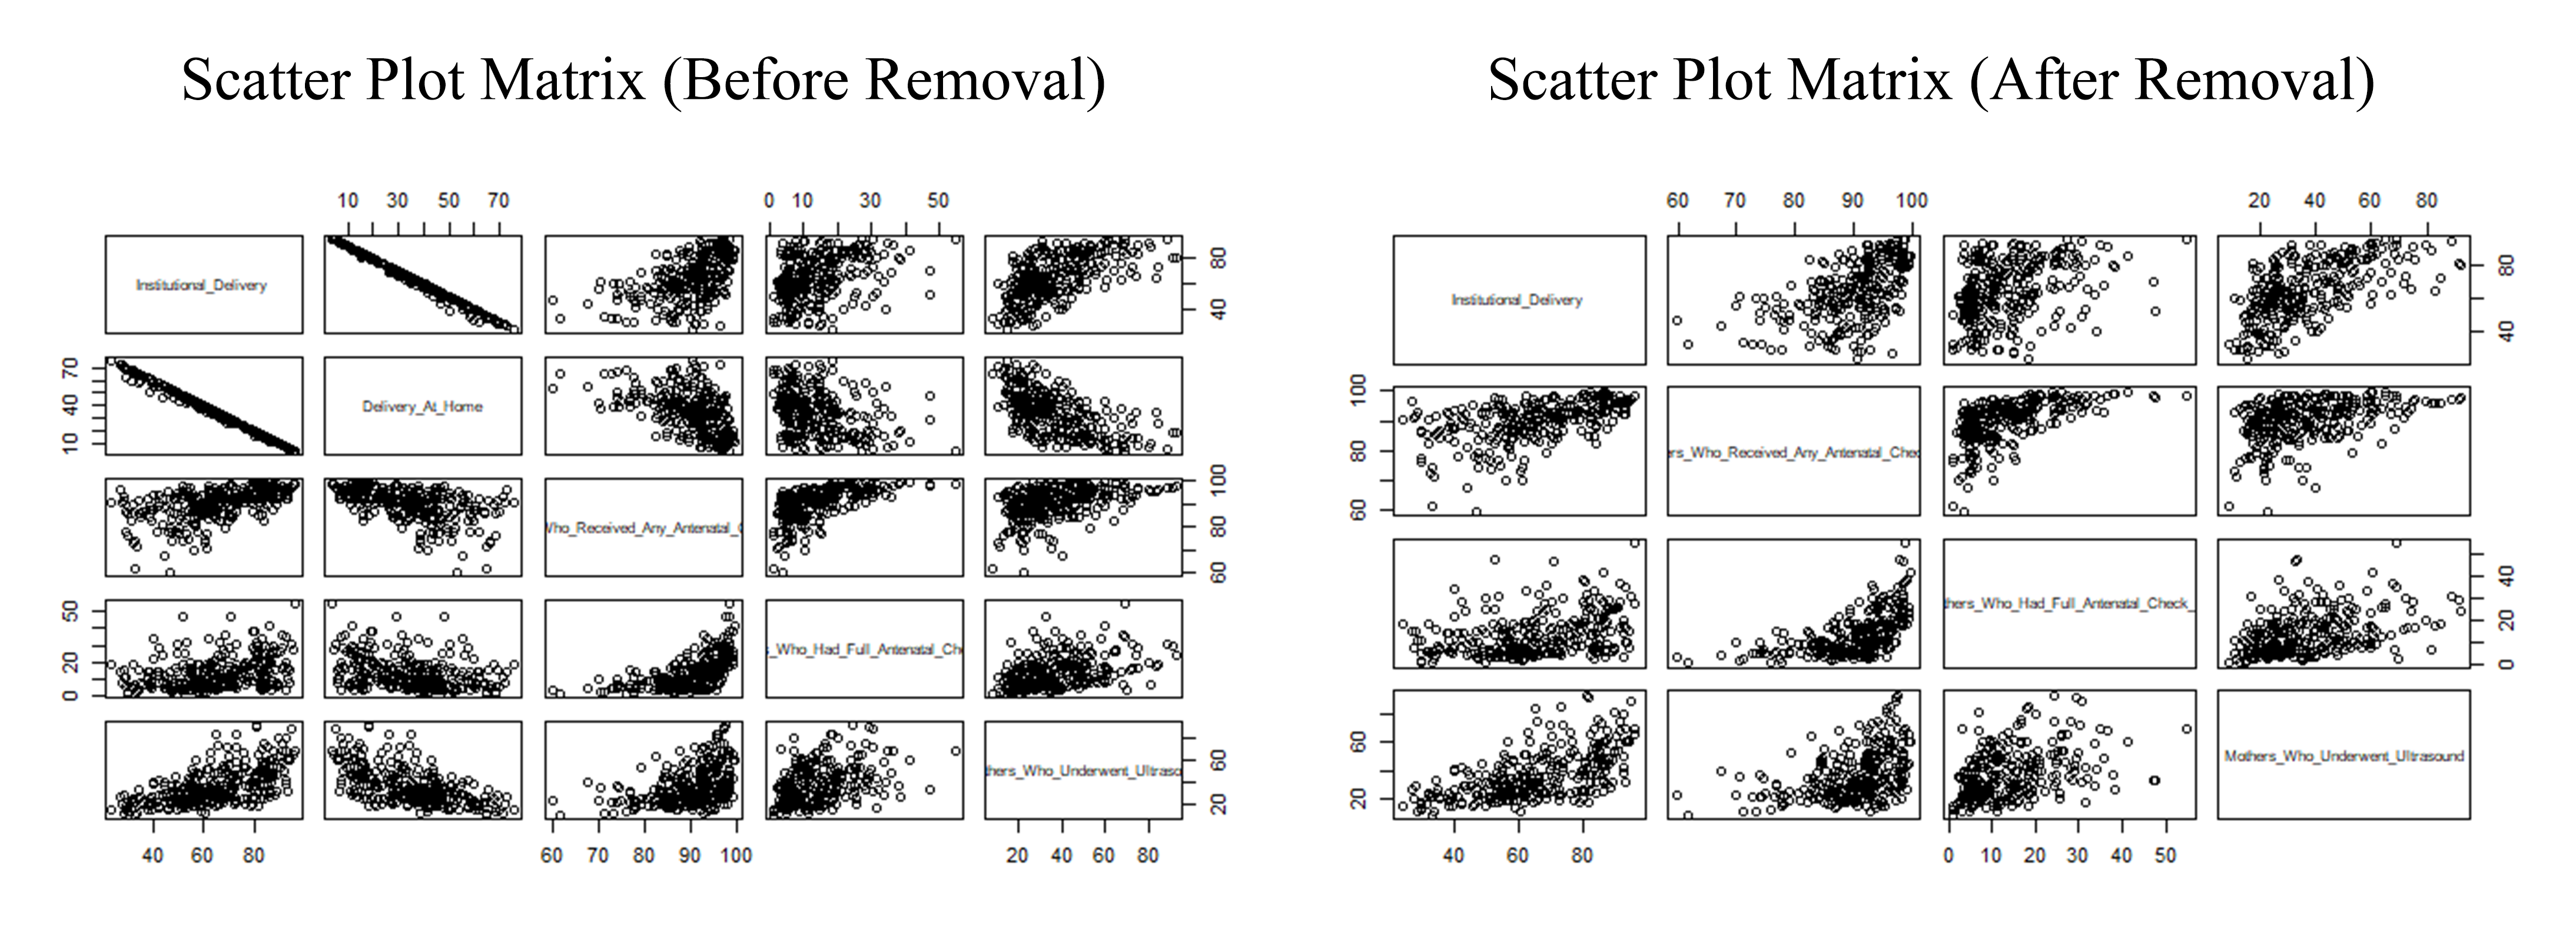
\includegraphics[width=1.0\textwidth]{scatterplotmatrix.png}
    \caption{\label{fig:}Scatter Plot Matrix, before and after}
\end{figure}
Afterward, an investigation on ``R squared,'' ``Adjusted R Squared,'' ``AIC,'' and ``BIC'' was conducted to analyze which model could yield the most accurate result. The investigation shows no good selections. Hence, LASSO and Stepwise Selection based on AIC and BIC were conducted. LASSO selection agrees with AIC-based selection, with all the remaining four predictors being preserved, while BIC-based selection eliminates one of the predictors. As the study aims to study the relationship, prediction is of secondary importance. The lesser variable is desired as it is interpretable. Therefore, the BIC-based selection result was used to fit the final model.

\subsection{Model validation}
During the validation phase of the analysis, cross-validation and prediction performance were conducted. 10-fold cross-validation was performed for LASSO, AIC-based, and BIC-based selection. The clean dataset was split into ten parts, and the model was fitted with nine training parts to predict the outcome of the remaining test part. All ten parts have been used as a test set. The prediction value was then plotted with the observed value to visualize the model's accuracy. A total of three prediction plots were generated for each LASSO selection, AIC-based selection, and BIC-based selection. In all three plots generated, we observe that the bias-corrected prediction differs from the ideal. We will discuss the potential cause of the difference and the limitation of the model in the last section. 

\subsection{Model violation and diagnostics}
Diagnostic checking was performed for both the univariate model and the multivariate model. First, a normal Q-Q plot was generated to ensure the Normality Assumption. The visualization of shows that the normality assumption is met for both models \ref{appendix:qq1}. Sample quantiles fluctuate a bit at both tails. However, the degree of fluctuation does not violate the normality assumption. Following the normal Q-Q plot, a standardized Residue vs. Predictor plot was generated to ensure the Linearity Assumption. Visualization of the predictor plot confirms that the assumption is met \ref{appendix:qq2}. Finally, a temporary model was fit using the square root of the absolute value of the residue. No clear pattern emerges in the plot, and we confirm that the homoscedasticity assumption is met. As mentioned in the previous sections, multicollinearity analysis was conducted for the multivariate model. One of the variables was removed due to almost perfect collinearity. Note that a Response vs. Fitted value plot for the multivariate model was generated to inspect if any transformation is needed. There is no obvious quadratic or logarithmic relation between the response and the predictor space. Hence, we conclude that transformation is not necessary.

\section{Results}
\subsection{Description of data}
\begin{table}[!ht]
\centering
\resizebox{\linewidth}{!}{%
\begin{tabular}{lcccccc} 
\hline\hline
Variable Name                                     & Variable Type & $min$  & Median & $max$  & $\mu$ & $\sigma^2$  \\ 
\hline
State\_Name                                       & Character     & N/A  & N/A    & N/A  & N/A  & N/A       \\
State\_District\_Name                             & Character     & N/A  & N/A    & N/A  & N/A  & N/A       \\
Mothers\_Who\_Received\_Any\_Antenatal\_Check\_Up & Decimal       & 59.9 & 91.7   & 99.7 & 90   & 6.9       \\
Mothers\_Who\_Had\_Full\_Antenatal\_Check\_Up     & Decimal       & 1    & 10.8   & 54.6 & 13.5 & 9.4       \\
Mothers\_Who\_Underwent\_Ultrasound               & Decimal       & 8.6  & 32.1   & 92.5 & 36.6 & 17        \\
Institutional\_Delivery                           & Decimal       & 23.8 & 64.3   & 95.9 & 64.8 & 17.3      \\
Delivery\_At\_Home                                & Decimal       & 4    & 34.3   & 75.9 & 34.3 & 16.9      \\
Infant\_Mortality\_Rate                           & Decimal       & 19.2 & 55     & 97   & 56.2 & 14.1      \\
\hline\hline
\end{tabular}
}
\caption{Summary of variables}
\end{table}
\noindent An exploratory data analysis was performed prior to the model analysis. A summary of each variable is presented in the table above. Missing values have been checked in all eight variables. The result shows that these variables are complete. This means that all eight variables have been filled for the entire 284 observations. Then, a histogram was plotted for the variable of interest and five predictors. These six continuous variables range from 0 to 100, representing percentages. Histogram has been generated for all six variables \ref{appendix:hist}. Next, the distribution of the three antenatal-related predictors was checked. ``Mothers Who Received Any Antenatal Check-Up'' has a negatively skewed distribution. ``Mothers Who Had Full Antenatal Check Up'' and ``Mothers Who Underwent Ultrasound'' have a positively skewed distribution. In most of the districts in India, most of the mothers received at least some sort of antenatal check-up, but only a few mothers received a full antenatal check. Both delivery method-related predictors have a distribution that resembles a normal distribution, except for the spike at 80-85\% in ``Institutional Delivery'' and the spike at 15-20\% in ``Delivery At Home.'' These two predictors are almost perfectly correlated as the percentage of institutional delivery and delivery at home adds up to 100\%.

\subsection{Analysis and results}
Two models have been fitted for this study, one being univariate, using the predictor ``Institutional Delivery,'' and one being multivariate, using all five predictors (with two being removed in the final model). Cook's distance was used in the leverage point and outliers analysis for the univariate model. DFFITS and DFBETAS were used in the multivariate model's leverage point and outliers analysis. As a result, 11 observation was removed from the univariate model, and 21 observations were removed from the multivariate model. After the removal of influential observations, both models were refitted. Second, the assumptions of linear models are checked; a normal Q-Q plot was used for checking normality \ref{appendix:qq1}, standardized Residue vs. Predictor plot was used for checking linearity \ref{appendix:qq2}.
\begin{figure}[!ht]
    \centering
    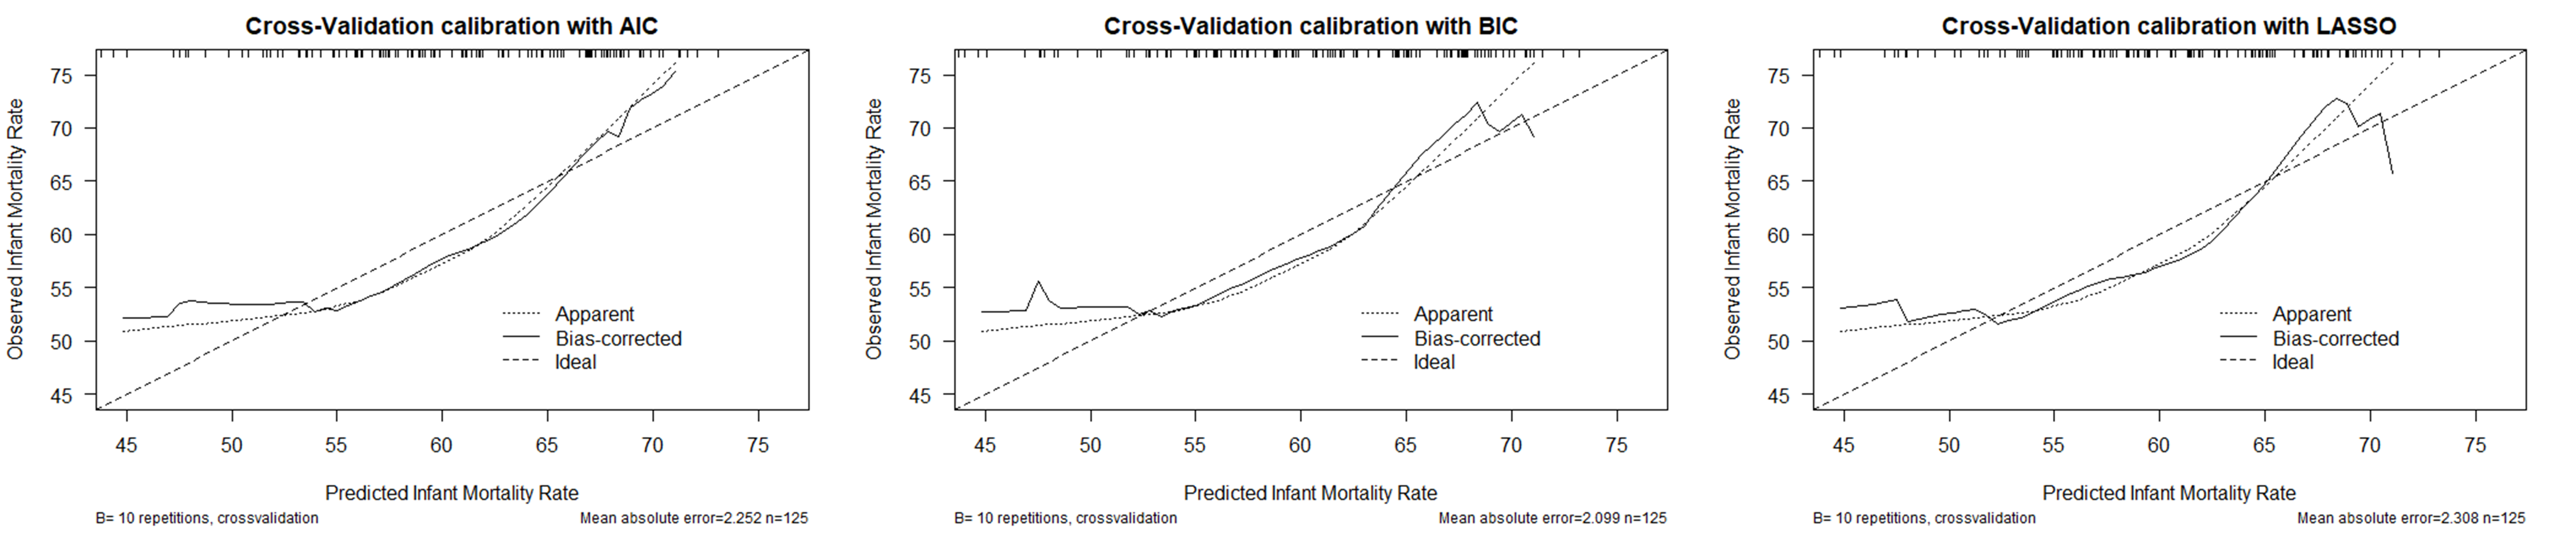
\includegraphics[width=1.0\textwidth]{cross validation.png}
    \caption{\label{fig:}Cross-Validation Calibration with AIC, BIC, and LASSO}
\end{figure}
The square root of the absolute value of the residue was used for checking homoscedasticity. For the multivariate model, multicollinearity and VIF analysis were conducted. Two of the predictors (Institutional Delivery and Delivery at Home) have a VIF of 137.611436 and 134.846212, respectively. These values far exceed the proposed threshold of 5. Hence, one of these two variables (Delivery at Home) was removed. Then, model selection was performed using LASSO selection, AIC-based selection, and BIC-based selection. The result from the BIC-based selection included three predictors and was selected as the final model. During the model validation, cross-validation was performed, and the mean squared error was calculated based on the previously mentioned three methods of selection. The result for mean squared error is 6.45618, 6.5517, and 8.92306, respectively. Note that the presence of error has a negligible effect on our study as our goal is not to predict but to study the relationship between predictors and variables of interest. Finally, a 95\% confidence interval was constructed based on the final model. The below table summarizes the final model fitted. An ANOVA test was conducted for both univariate and multivariate models. In the univariate model, we failed to reject the null hypothesis ($\mathcal{F}$-value=0.4650763). In the multivariate model, we failed to reject the null hypothesis for the predictor ``Institutional Delivery'' ($\mathcal{F}$-value=0.016) and rejected the null hypothesis for the other two predictors, ``Mothers Who Received Any Antenatal Check Up'' ($\mathcal{F}$-value=27.773) and ``Mothers Who Underwent Ultrasound'' ($\mathcal{F}$-value=32.772).  
\begin{table}[!ht]
\centering
\resizebox{\linewidth}{!}{%
\begin{tabular}{lccccccc} 
\hline\hline
                                              & Estimate          & Std. Error       & $t$-value & df  & Sum Sq & Mean Sq & $\mathcal{F}$-value          \\ 
\hline
\textbf{Univariate Model}                     &                   &                  &             &     &        &         &                  \\
~ (Intercept)                                 & 54.31161          & 3.13525          & 17.323      &     &        &         &                  \\
~ Institutional Delivery                      & \textbf{0.03163}  & \textbf{0.04639} & 0.682       & 1   & 77     & 77.271  & \textbf{0.4651}  \\
~ Residuals                                   &                   &                  &             & 271 & 45026  & 166.146 &                  \\
\textbf{Multivariate Model}                   &                   &                  &             &     &        &         &                  \\
~ (Intercept)                                 & 98.73380          & 9.59736          & 10.288      &     &        &         &                  \\
~ Institutional Delivery                      & \textbf{0.29644}  & \textbf{0.05578} & 5.314       & 1   & 2      & 2.0     & \textbf{0.016}   \\
~ Mothers Who Received Any Antenatal Check Up & \textbf{-0.56311} & \textbf{0.12001} & -4.692      & 1   & 3427   & 3427.3  & \textbf{27.773}  \\
~ Mothers Who Underwent Ultrasound            & \textbf{-0.30168} & \textbf{0.05270} & -5.725      & 1   & 4044   & 4044.1  & \textbf{32.772}  \\
~ Residuals                                   &                   &                  &             & 259 & 31961  & 123.4   &                  \\
\hline\hline
\end{tabular}
}
\caption{Model summary combined with ANOVA table}
\end{table}

\section{Discussion}
Both the univariate model and multivariate model failed to reject the null hypothesis. The null hypothesis tested is $\beta_1=1$. We can interpret this as ``When conditioned on the percentage of Institutional Delivery, Infant Mortality Rate will not change.'' Hence, we can conclude that there is no relationship between ``Institutional Delivery'' and ``Infant Mortality Rate.'' For the multivariate model, we failed to reject the null hypothesis for the other two predictors. Surprisingly, the estimate (-0.56311 $\pm$ 0.12001 and -0.30168 $\pm$ 0.05) indicates a negative relation. Note that during the model validation phase, we noticed a prediction error. This might be caused by the limitation of the dataset, as the nine states modeled in this study accounts for only 48\% of the total Indian population, and the fertility and mortality in these states are relatively higher than in the other states in India. A potential solution would be to gather the data from the other 52\% of the population. Our research concludes that if a country wishes to decrease the Infant Mortality rate efficiently, Institutional Delivery takes less importance, while other factors should be considered as a priority. 

\bibliographystyle{ieeetr}
\bibliography{ref}

\appendix

\section{Appendix: Q-Q plot and Residue vs. Predictor plot}
\label{appendix:qq1}
\begin{figure}[!ht]
    \centering
    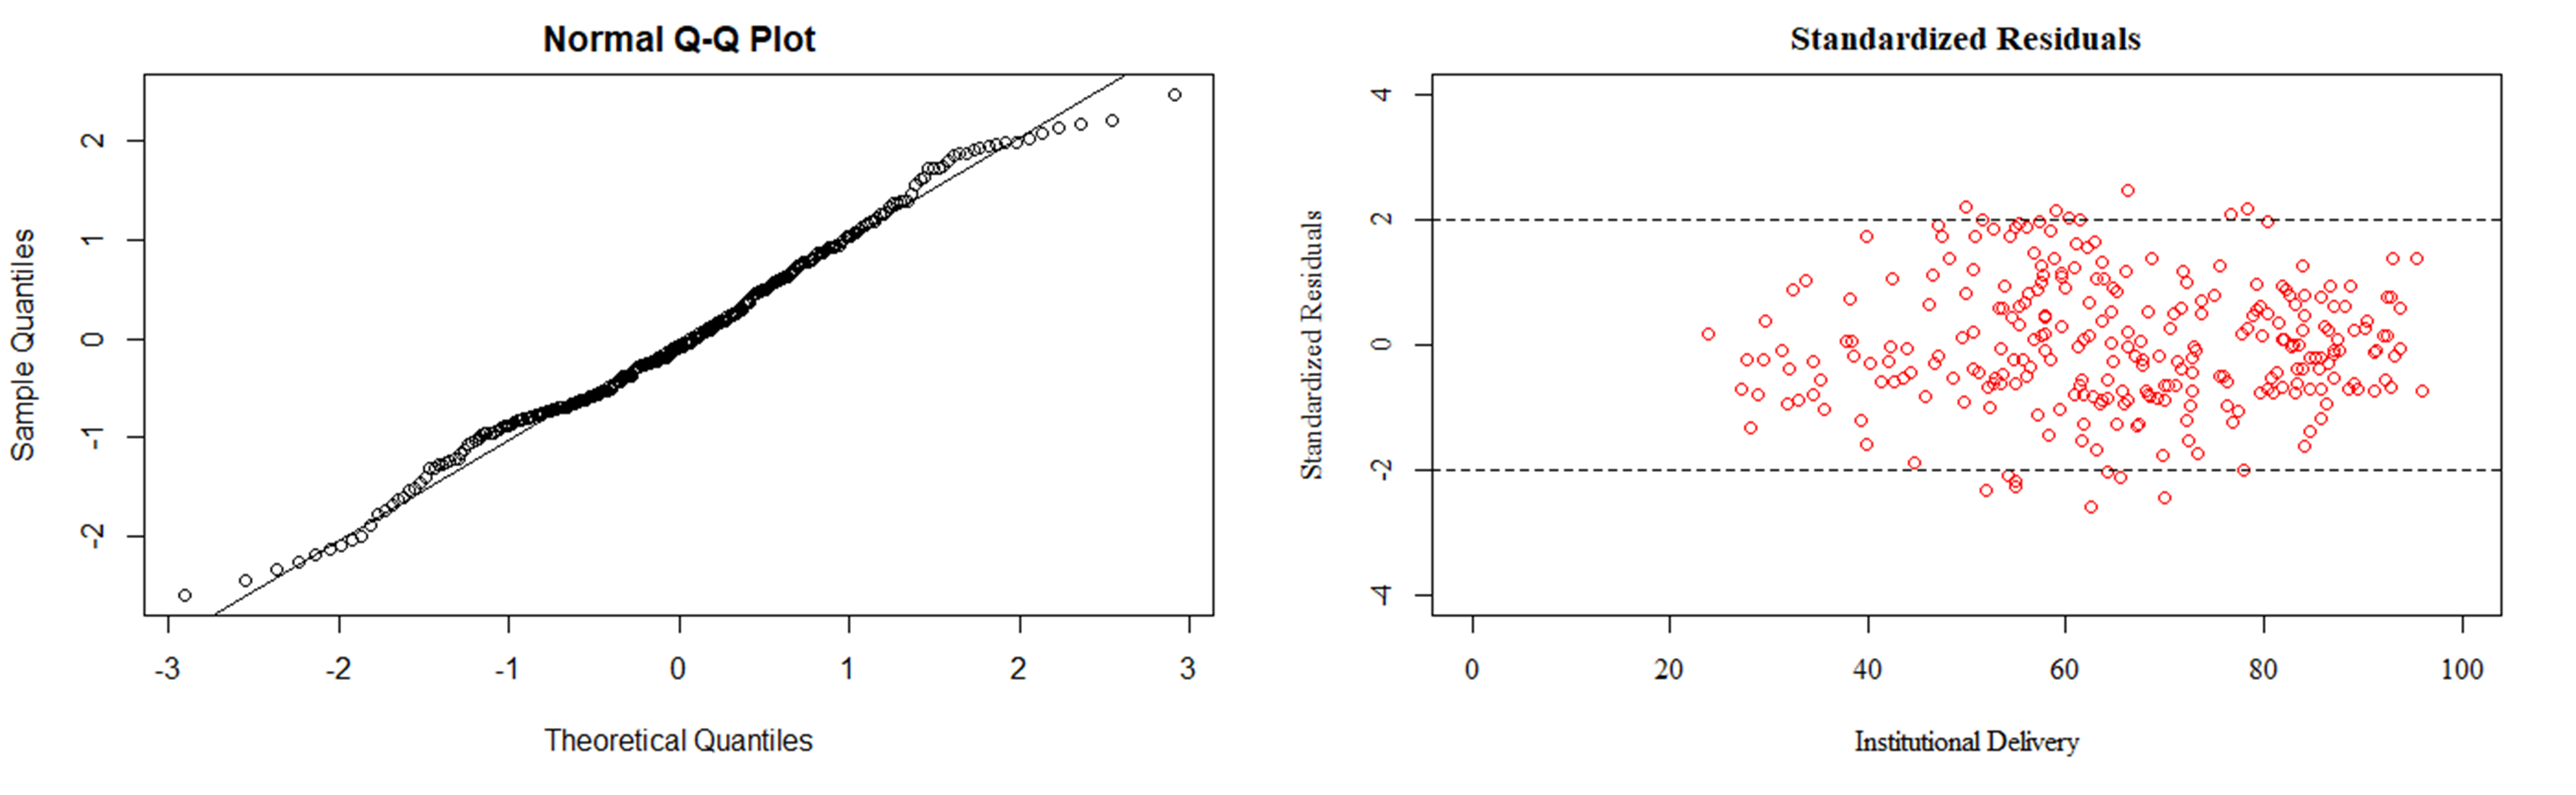
\includegraphics[width=0.7\textwidth]{qq+res uni.png}
    \caption{\label{fig:}Q-Q plot and Residue vs. Predictor plot (univariate model)}
\end{figure}

\label{appendix:qq2}
\begin{figure}[!ht]
    \centering
    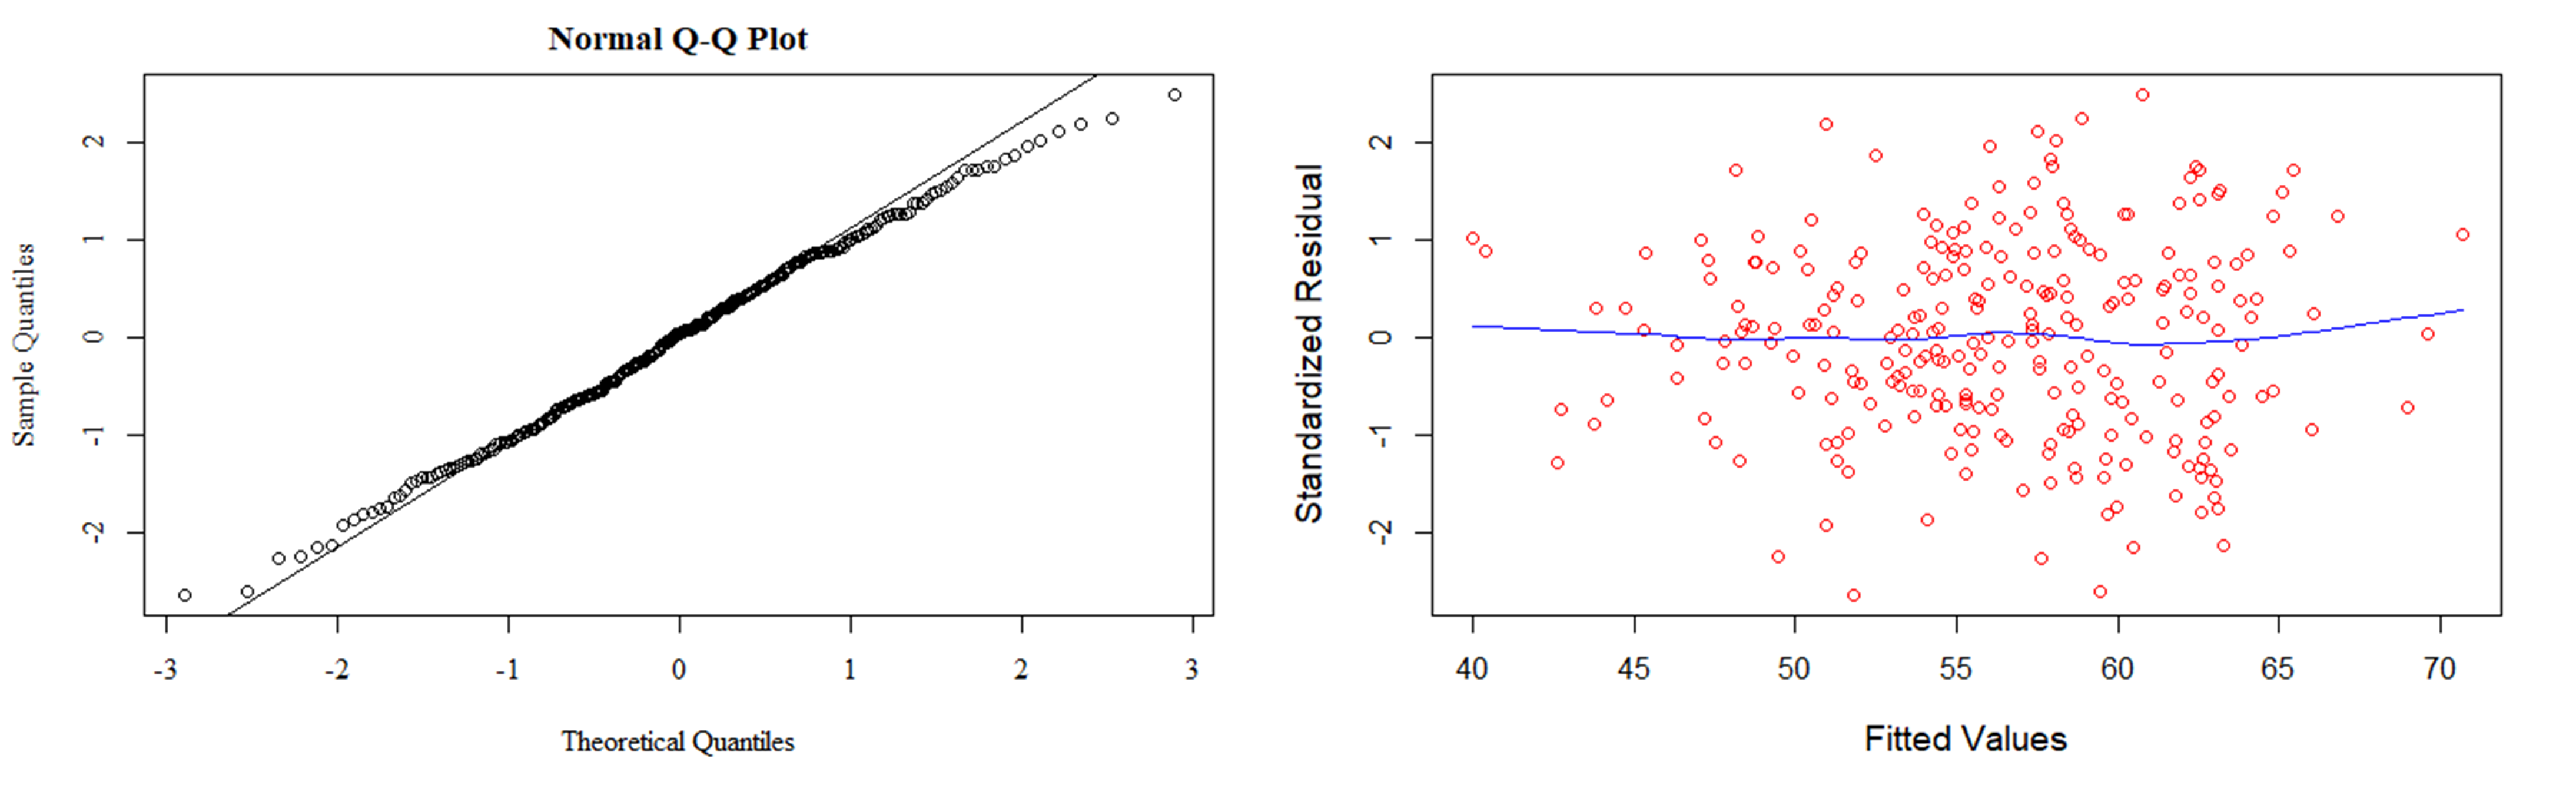
\includegraphics[width=0.7\textwidth]{qq+res multi.png}
    \caption{\label{fig:}Q-Q plot and Residue vs. Predictor plot (multivariate model)}
\end{figure}

\section{Appendix: Histogram generated during EDA}
\label{appendix:hist}
\begin{figure}[!ht]
    \centering
    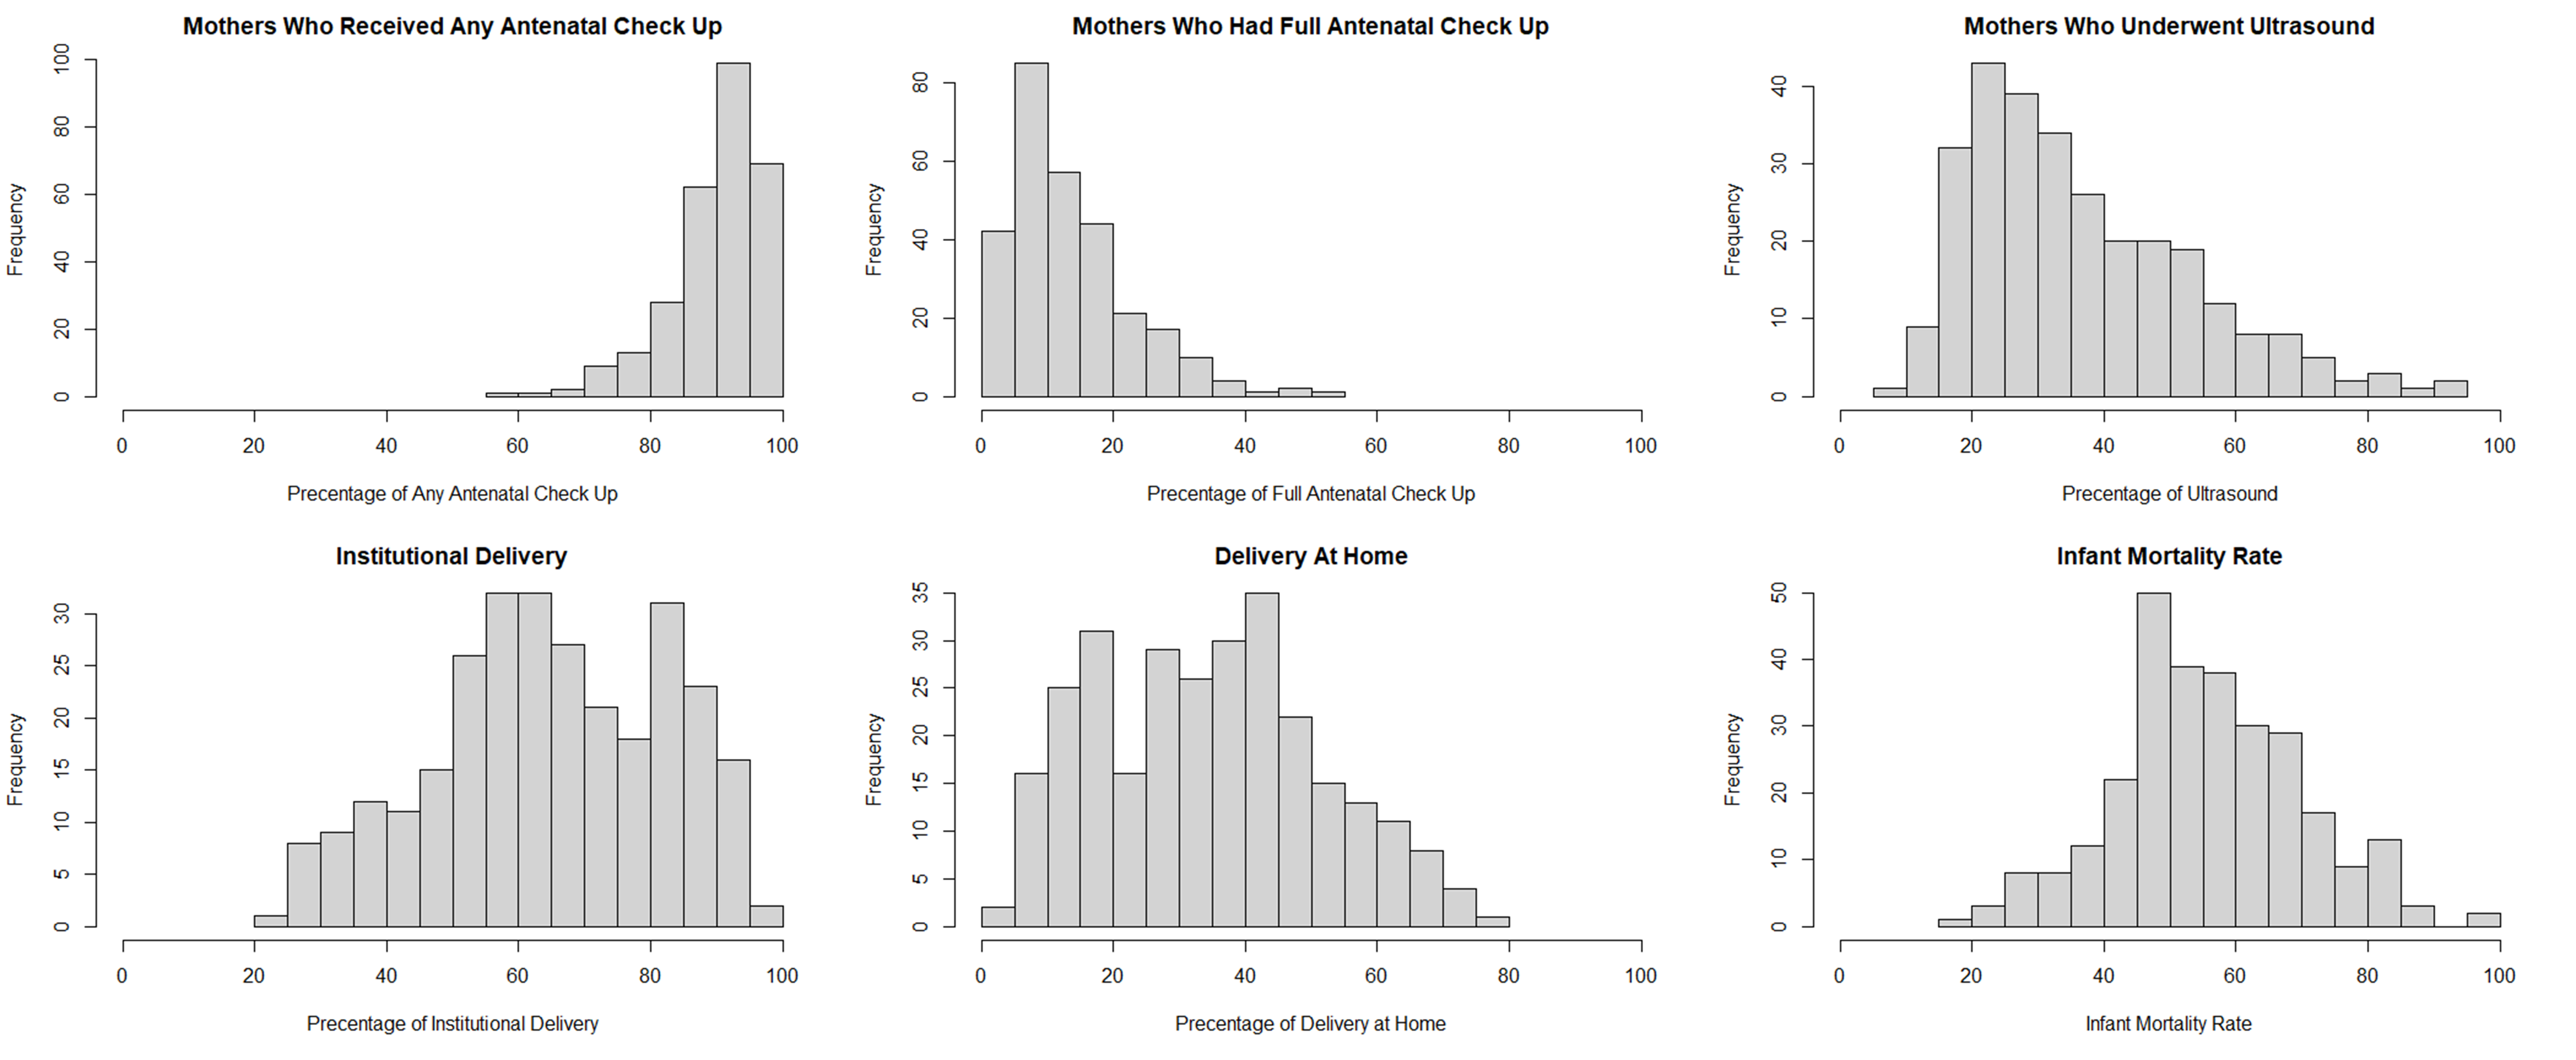
\includegraphics[width=0.7\textwidth]{EDA.png}
    \caption{\label{fig:}Histogram of five predictors and variable of interest}
\end{figure}

\end{document}